\cleardoublepage
\chapter{Resultados}
\label{chap:resultados}

Este capítulo recoge los resultados obtenidos tras el desarrollo y validación de WebBuilder, presentando el sistema como producto terminado y resumiendo las funcionalidades conseguidas.

\section{WebBuilder como plataforma}
\label{sec:webbuilder-plataforma}

Al finalizar el desarrollo de WebBuilder se han implementado y validado con éxito las siguientes funcionalidades:

\begin{itemize}
    \item Análisis automático de APIs públicas en los formatos JSON, XML, CSV y GeoJSON, con detección del esquema de datos mediante LLM y validación anti-alucinaciones.
    \item Generación completa de proyectos Django funcionales en siete pasos coordinados por el LLM, incluyendo modelos, vistas, plantillas, carga de datos y configuración de despliegue.
    \item Despliegue automático de los proyectos generados en contenedores Docker independientes mediante flujos de trabajo en n8n, devolviendo una URL de previsualización al usuario.
    \item Soporte para múltiples proveedores de modelos de lenguaje mediante el estándar OpenAI-compatible, con un catálogo de modelos preconfigurados y la posibilidad de conectar un proveedor personalizado.
    \item Sistema de trazabilidad completo con registro de cada llamada al LLM, verificación de consistencia del código generado y panel de métricas para administradores.
    \item Historial de versiones por proyecto, con posibilidad de redesplegar cualquier versión anterior, descargar el código fuente y refinar el sitio con el asistente de IA.
    \item Interfaz bilingüe (español e inglés) con modo claro y oscuro, accesible desde cualquier navegador sin instalación de software adicional.
\end{itemize}

\begin{figure}[H]
    \centering
    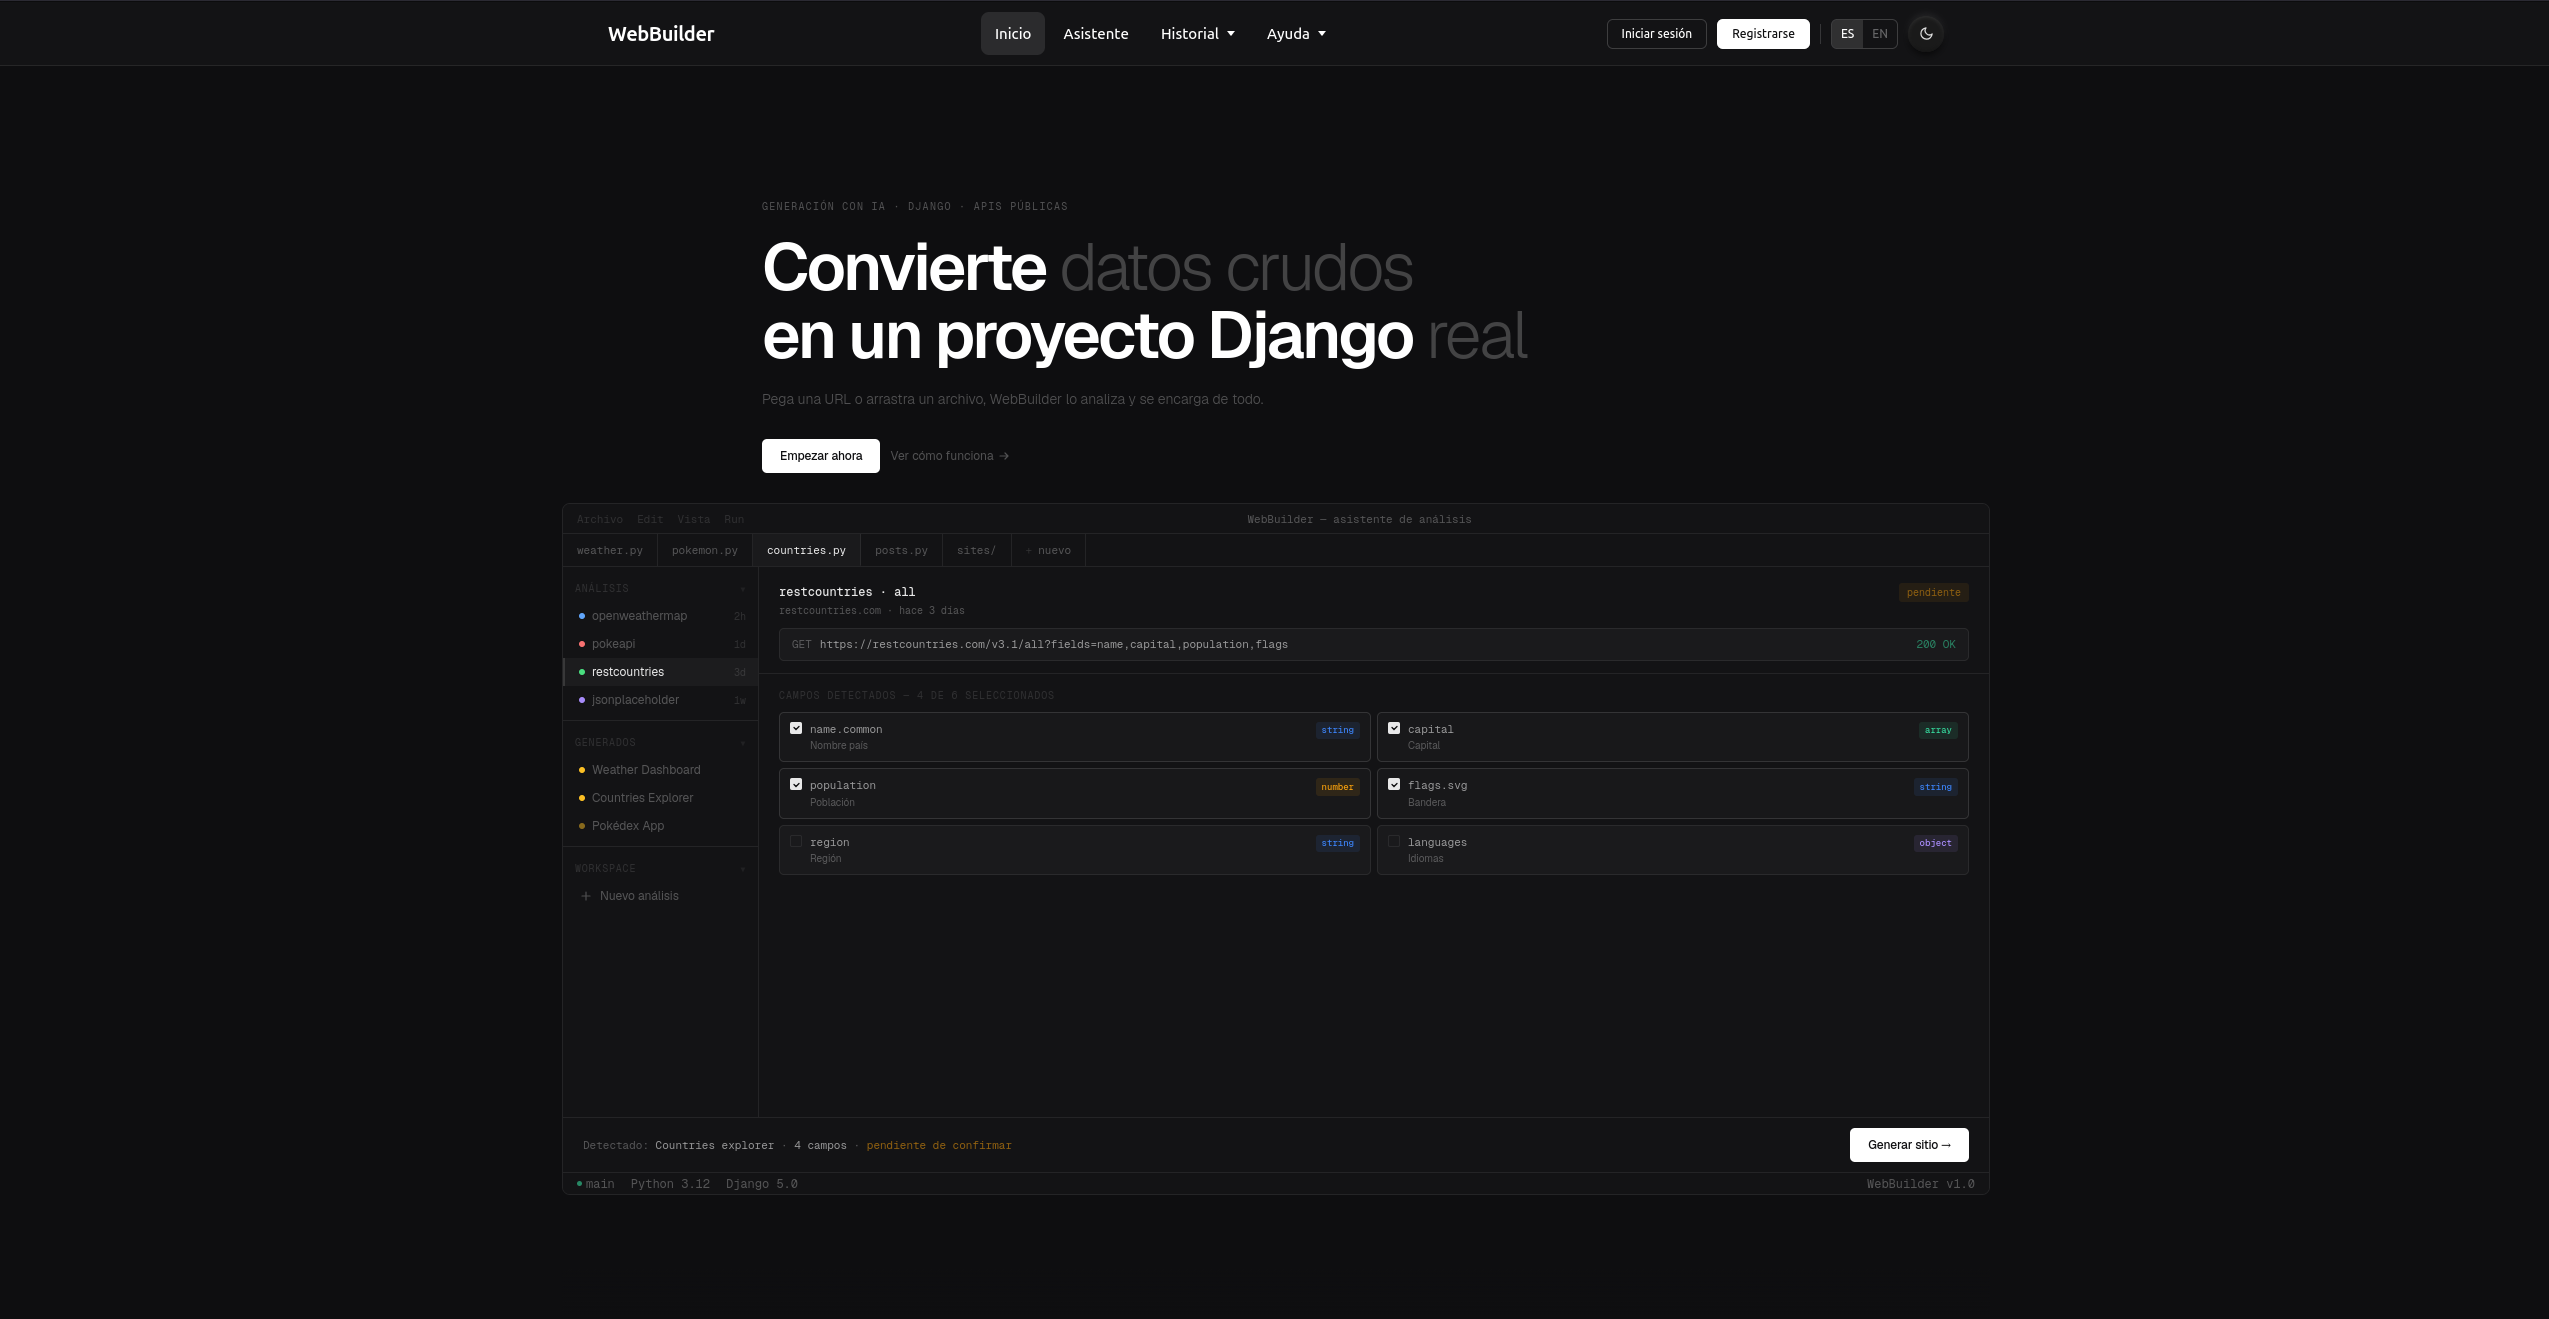
\includegraphics[width=\textwidth]{img/webbuilder/hero.png}
    \caption{Página principal de WebBuilder}
    \label{fig:wb-home}
\end{figure}

\section{Resultados casos de uso}
\label{sec:casos-uso-resultados}

Como demostración del funcionamiento real del sistema, se generaron tres sitios web completos a partir de APIs públicas de distinta naturaleza, cuyos resultados se describen en detalle en el Capítulo~\ref{chap:experimentos}. Los tres proyectos fueron generados de forma automática, desplegados en contenedores Docker independientes y validados según los criterios definidos en la metodología de validación.

El primer caso utilizó la API de TheCocktailDB para generar una web de recetas de cócteles con catálogo visual paginado y páginas de detalle. El segundo caso utilizó la API de SampleAPIs para generar un catálogo de películas de animación con pósters e información de cada título. El tercer caso utilizó la API de Rick and Morty para generar un catálogo de personajes con imágenes, badges de estado y páginas de detalle estructuradas.

Los tres casos demuestran que WebBuilder es capaz de adaptarse a tipos de datos y estilos visuales completamente distintos sin ninguna configuración adicional más allá del prompt inicial del usuario.

\section{Disponibilidad del software}
\label{sec:disponibilidad}

El código fuente de WebBuilder está disponible públicamente en el 
siguiente repositorio de GitHub:

\begin{center}
\url{https://github.com/AlejandroTejero/WebBuilder-TFG}
\end{center}

El proyecto se distribuye bajo la licencia \textbf{CC0 1.0 Universal} 
(\emph{Creative Commons Zero}), la cual equivale a subir el proyecto a dominio público. Esto 
significa que cualquier persona puede usar, modificar, distribuir o 
incorporar el código en el proyecto, sin necesidad de solicitar permiso al autor original. Contribuyendo de esta forma al ecosistema de aplicaciones de código abierto.

La landing page del proyecto, que actúa como página informativa y de documentación, 
se encuentra en el Apéndice~\ref{app:manual}.